% Options for packages loaded elsewhere
\PassOptionsToPackage{unicode}{hyperref}
\PassOptionsToPackage{hyphens}{url}
\PassOptionsToPackage{dvipsnames,svgnames,x11names}{xcolor}
%
\documentclass[
  a4paper,
]{article}

\usepackage{amsmath,amssymb}
\usepackage{iftex}
\ifPDFTeX
  \usepackage[T1]{fontenc}
  \usepackage[utf8]{inputenc}
  \usepackage{textcomp} % provide euro and other symbols
\else % if luatex or xetex
  \usepackage{unicode-math}
  \defaultfontfeatures{Scale=MatchLowercase}
  \defaultfontfeatures[\rmfamily]{Ligatures=TeX,Scale=1}
\fi
\usepackage{lmodern}
\ifPDFTeX\else  
    % xetex/luatex font selection
    \setmainfont[]{Latin Modern Roman}
    \setsansfont[]{Latin Modern Sans}
    \setmonofont[]{Latin Modern Mono}
\fi
% Use upquote if available, for straight quotes in verbatim environments
\IfFileExists{upquote.sty}{\usepackage{upquote}}{}
\IfFileExists{microtype.sty}{% use microtype if available
  \usepackage[]{microtype}
  \UseMicrotypeSet[protrusion]{basicmath} % disable protrusion for tt fonts
}{}
\makeatletter
\@ifundefined{KOMAClassName}{% if non-KOMA class
  \IfFileExists{parskip.sty}{%
    \usepackage{parskip}
  }{% else
    \setlength{\parindent}{0pt}
    \setlength{\parskip}{6pt plus 2pt minus 1pt}}
}{% if KOMA class
  \KOMAoptions{parskip=half}}
\makeatother
\usepackage{xcolor}
\setlength{\emergencystretch}{3em} % prevent overfull lines
\setcounter{secnumdepth}{-\maxdimen} % remove section numbering
% Make \paragraph and \subparagraph free-standing
\makeatletter
\ifx\paragraph\undefined\else
  \let\oldparagraph\paragraph
  \renewcommand{\paragraph}{
    \@ifstar
      \xxxParagraphStar
      \xxxParagraphNoStar
  }
  \newcommand{\xxxParagraphStar}[1]{\oldparagraph*{#1}\mbox{}}
  \newcommand{\xxxParagraphNoStar}[1]{\oldparagraph{#1}\mbox{}}
\fi
\ifx\subparagraph\undefined\else
  \let\oldsubparagraph\subparagraph
  \renewcommand{\subparagraph}{
    \@ifstar
      \xxxSubParagraphStar
      \xxxSubParagraphNoStar
  }
  \newcommand{\xxxSubParagraphStar}[1]{\oldsubparagraph*{#1}\mbox{}}
  \newcommand{\xxxSubParagraphNoStar}[1]{\oldsubparagraph{#1}\mbox{}}
\fi
\makeatother


\providecommand{\tightlist}{%
  \setlength{\itemsep}{0pt}\setlength{\parskip}{0pt}}\usepackage{longtable,booktabs,array}
\usepackage{calc} % for calculating minipage widths
% Correct order of tables after \paragraph or \subparagraph
\usepackage{etoolbox}
\makeatletter
\patchcmd\longtable{\par}{\if@noskipsec\mbox{}\fi\par}{}{}
\makeatother
% Allow footnotes in longtable head/foot
\IfFileExists{footnotehyper.sty}{\usepackage{footnotehyper}}{\usepackage{footnote}}
\makesavenoteenv{longtable}
\usepackage{graphicx}
\makeatletter
\newsavebox\pandoc@box
\newcommand*\pandocbounded[1]{% scales image to fit in text height/width
  \sbox\pandoc@box{#1}%
  \Gscale@div\@tempa{\textheight}{\dimexpr\ht\pandoc@box+\dp\pandoc@box\relax}%
  \Gscale@div\@tempb{\linewidth}{\wd\pandoc@box}%
  \ifdim\@tempb\p@<\@tempa\p@\let\@tempa\@tempb\fi% select the smaller of both
  \ifdim\@tempa\p@<\p@\scalebox{\@tempa}{\usebox\pandoc@box}%
  \else\usebox{\pandoc@box}%
  \fi%
}
% Set default figure placement to htbp
\def\fps@figure{htbp}
\makeatother
% definitions for citeproc citations
\NewDocumentCommand\citeproctext{}{}
\NewDocumentCommand\citeproc{mm}{%
  \begingroup\def\citeproctext{#2}\cite{#1}\endgroup}
\makeatletter
 % allow citations to break across lines
 \let\@cite@ofmt\@firstofone
 % avoid brackets around text for \cite:
 \def\@biblabel#1{}
 \def\@cite#1#2{{#1\if@tempswa , #2\fi}}
\makeatother
\newlength{\cslhangindent}
\setlength{\cslhangindent}{1.5em}
\newlength{\csllabelwidth}
\setlength{\csllabelwidth}{3em}
\newenvironment{CSLReferences}[2] % #1 hanging-indent, #2 entry-spacing
 {\begin{list}{}{%
  \setlength{\itemindent}{0pt}
  \setlength{\leftmargin}{0pt}
  \setlength{\parsep}{0pt}
  % turn on hanging indent if param 1 is 1
  \ifodd #1
   \setlength{\leftmargin}{\cslhangindent}
   \setlength{\itemindent}{-1\cslhangindent}
  \fi
  % set entry spacing
  \setlength{\itemsep}{#2\baselineskip}}}
 {\end{list}}
\usepackage{calc}
\newcommand{\CSLBlock}[1]{\hfill\break\parbox[t]{\linewidth}{\strut\ignorespaces#1\strut}}
\newcommand{\CSLLeftMargin}[1]{\parbox[t]{\csllabelwidth}{\strut#1\strut}}
\newcommand{\CSLRightInline}[1]{\parbox[t]{\linewidth - \csllabelwidth}{\strut#1\strut}}
\newcommand{\CSLIndent}[1]{\hspace{\cslhangindent}#1}

\usepackage{booktabs}
\usepackage{longtable}
\usepackage{array}
\usepackage{multirow}
\usepackage{wrapfig}
\usepackage{float}
\usepackage{colortbl}
\usepackage{pdflscape}
\usepackage{tabu}
\usepackage{threeparttable}
\usepackage{threeparttablex}
\usepackage[normalem]{ulem}
\usepackage{makecell}
\usepackage{xcolor}
\usepackage{fancyhdr}
\pagestyle{fancy}
\fancyhf{}
\fancyhead[L]{\nouppercase{\leftmark}}
\fancyhead[R]{\thepage}
\renewcommand{\headrulewidth}{0.4pt}
\usepackage[margin=2.5cm]{geometry}
\makeatletter
\@ifpackageloaded{caption}{}{\usepackage{caption}}
\AtBeginDocument{%
\ifdefined\contentsname
  \renewcommand*\contentsname{Table of contents}
\else
  \newcommand\contentsname{Table of contents}
\fi
\ifdefined\listfigurename
  \renewcommand*\listfigurename{List of Figures}
\else
  \newcommand\listfigurename{List of Figures}
\fi
\ifdefined\listtablename
  \renewcommand*\listtablename{List of Tables}
\else
  \newcommand\listtablename{List of Tables}
\fi
\ifdefined\figurename
  \renewcommand*\figurename{Figure}
\else
  \newcommand\figurename{Figure}
\fi
\ifdefined\tablename
  \renewcommand*\tablename{Table}
\else
  \newcommand\tablename{Table}
\fi
}
\@ifpackageloaded{float}{}{\usepackage{float}}
\floatstyle{ruled}
\@ifundefined{c@chapter}{\newfloat{codelisting}{h}{lop}}{\newfloat{codelisting}{h}{lop}[chapter]}
\floatname{codelisting}{Listing}
\newcommand*\listoflistings{\listof{codelisting}{List of Listings}}
\makeatother
\makeatletter
\makeatother
\makeatletter
\@ifpackageloaded{caption}{}{\usepackage{caption}}
\@ifpackageloaded{subcaption}{}{\usepackage{subcaption}}
\makeatother

\usepackage{bookmark}

\IfFileExists{xurl.sty}{\usepackage{xurl}}{} % add URL line breaks if available
\urlstyle{same} % disable monospaced font for URLs
\hypersetup{
  pdftitle={Master Thesis},
  pdfkeywords={Phosphorus release kinetics, Fertiizer requirements
prediction},
  colorlinks=true,
  linkcolor={blue},
  filecolor={Maroon},
  citecolor={Blue},
  urlcolor={Blue},
  pdfcreator={LaTeX via pandoc}}


\title{Master Thesis}
\author{Marc Pérez}
\date{}

\begin{document}
\maketitle
\begin{abstract}
Hier kommt das Abstract
\end{abstract}


\section{Preface}\label{preface}

\section{Abstract}\label{abstract}

(Knuth 1984)

\section{Introduction}\label{introduction}

\subsection{The Complexity of
Phosphorus}\label{the-complexity-of-phosphorus}

Phosphorus (P) is an essential macronutrient for all known life, forming
a critical part of DNA and energy-transfer molecules. In soils---where
organic, mineral, and aqueous phases interface---its behavior is
complex. In the presence of oxygen, P exists almost exclusively as
orthophosphate (\(PO_4^{3-}\)) and its protonated forms (\(HPO_4^{2-}\)
or \(H_2PO_4^{-}\)), depending on the soil pH. These dissolved phosphate
species are highly reactive; they are subject to adsorption onto the
surfaces of clays and oxides and can precipitate with cations like
calcium, iron, and aluminum to form minerals with low solubility.
Consequently, while the total amount of P in a soil can be large, only a
small fraction is in the soil solution at any given moment, posing a
central challenge for agriculture. The efficacy of P fertilization is
often low due to these rapid immobilization processes, and P lost from
agricultural fields can become an environmental pollutant, disturbing
P-limited aquatic ecosystems.

\textbf{Soil organic matter (SOM) adds another layer of complexity to
these interactions.} Organic acids released during the decomposition of
SOM can compete with phosphate for the same adsorption sites on mineral
surfaces, which can increase P concentrations in the soil solution.
Furthermore, humic substances can form stable complexes with cations
like Al³⁺ and Fe³⁺, preventing them from precipitating phosphate and
thereby enhancing its availability. The efficacy of P fertilization is
often low due to these rapid and competing immobilization processes, and
P lost from agricultural fields can become an environmental pollutant,
disturbing P-limited aquatic ecosystems. \#\# From Static Measurements
to Dynamic Understanding

To manage this challenge, traditional soil testing methods (e.g.,
Olsen-P, AAE10, CO₂-water) were developed to quantify the \textbf{size
of the readily available P pool}. This static measurement is often
referred to as the \textbf{``capacity factor''}. While these tests are
invaluable for basic fertility assessment, they do not capture the
dynamic nature of P supply. A crucial missing piece of information is
the rate at which P is replenished into the soil solution from the solid
phase after being taken up by plant roots. This replenishment rate, or
\textbf{``kinetic factor''}, is vital for sustaining crop growth,
especially during periods of high demand.

The importance of these dynamics is not a new concept. As early as 1982,
\textbf{Flossmann and Richter} argued that characterizing the kinetics
of P release was essential for refining fertilizer recommendations
beyond what static tests alone could offer. Modern research has
reinforced this view, showing that fertilization strategies based solely
on maintaining a critical soil test P (STP) concentration can be
inefficient. In Switzerland, this has led to the accumulation of
``legacy P'' in many agricultural soils, and understanding the release
kinetics of this legacy P is key to both improving nutrient efficiency
and protecting water quality. Furthermore, critical STP levels are not
constant; they are influenced by pedoclimatic factors like soil texture
and temperature, making a ``one-size-fits-all'' approach to
fertilization suboptimal.

\subsection{Objectives and Research
Questions}\label{objectives-and-research-questions}

An ideal set of parameters for P management should meet several
criteria. The parameters should correlate strongly with P export and P
balance in a steady-state system. They must also respond to fertilizer
inputs and, most importantly, capture the diffusive, kinetic nature of P
supply to plant roots.

This thesis hypothesizes that \textbf{kinetic parameters describing P
desorption, derived from a simple laboratory extraction, can serve as
effective predictors for agronomic outcomes.} Using soils from the
long-term STYCS experiment in Switzerland, this study employs a modified
version of the Flossmann \& Richter kinetic test to derive the
desorption rate (\(k\)) and the desorbable P pool (\(P^S\)). The
performance of these new kinetic parameters will be compared against
standard STP methods (\(P_{CO_2}\) and \(P_{AAE10}\)) by addressing the
following research questions:

\begin{enumerate}
\def\labelenumi{\arabic{enumi}.}
\tightlist
\item
  Is the P desorption kinetic method replicable and effective for the
  soils from the STYCS trial?
\item
  How do the kinetic coefficients, \(k\) and \(P^S\), correlate with key
  soil properties (organic carbon, clay content, pH)?
\item
  How well do the standard STP methods (\(P_{CO_2}\) \& \(P_{AAE10}\))
  predict crop yield, P export, and P balance?
\item
  Can the kinetic parameters, \(k\) and \(P^S\), improve the prediction
  of these agronomic outcomes compared to the standard static tests?
\end{enumerate}

\section{Materials and Methods}\label{materials-and-methods}

\subsection{The Long-Term Phosphorus Fertilization
Experiment}\label{the-long-term-phosphorus-fertilization-experiment}

The soil samples for this thesis originate from a set of six long-term
field trials in Switzerland, established by Agroscope between 1989 and
1992. The primary objective of these experiments was to validate and
re-evaluate Swiss phosphorus (P) fertilization guidelines by assessing
long-term crop yield responses to varying P inputs across different
pedoclimatic conditions. A detailed description of the experimental
design and site characteristics can be found in Hirte et al.~(2021).

The experiment was set up as a \textbf{completely randomized block
design} with four field replications at each site. The core of the
experiment consists of six fixed-plot treatments representing different
P fertilization levels, which were applied annually as superphosphate
before tillage and sowing. These levels were based on percentages of the
officially recommended P inputs: 0\% (Zero), 33\% (Deficit), 67\%
(Reduced), 100\% (Norm), 133\% (Elevated), and 167\% (Surplus).

\subsection{Experimental Sites}\label{experimental-sites}

The six experimental sites are located in the main crop-growing regions
of Switzerland: \textbf{Rümlang-Altwi (ALT)}, \textbf{Cadenazzo (CAD)},
\textbf{Ellighausen (ELL)}, \textbf{Grabs (GRA)}, \textbf{Oensingen
(OEN)}, and \textbf{Zurich-Reckenholz (REC)}. The key soil properties
are summarized below.

\begin{longtable}[]{@{}
  >{\raggedright\arraybackslash}p{(\linewidth - 10\tabcolsep) * \real{0.0704}}
  >{\raggedright\arraybackslash}p{(\linewidth - 10\tabcolsep) * \real{0.3099}}
  >{\raggedleft\arraybackslash}p{(\linewidth - 10\tabcolsep) * \real{0.1268}}
  >{\raggedleft\arraybackslash}p{(\linewidth - 10\tabcolsep) * \real{0.1268}}
  >{\raggedleft\arraybackslash}p{(\linewidth - 10\tabcolsep) * \real{0.2394}}
  >{\raggedleft\arraybackslash}p{(\linewidth - 10\tabcolsep) * \real{0.1268}}@{}}

\caption{\label{tbl-sites-corrected}Soil characteristics of the six
long-term experimental sites. Data adapted from Hirte et al.~(2021).}

\tabularnewline

\toprule\noalign{}
\begin{minipage}[b]{\linewidth}\raggedright
Site
\end{minipage} & \begin{minipage}[b]{\linewidth}\raggedright
Soil Type (WRB)
\end{minipage} & \begin{minipage}[b]{\linewidth}\raggedleft
Clay (\%)
\end{minipage} & \begin{minipage}[b]{\linewidth}\raggedleft
Sand (\%)
\end{minipage} & \begin{minipage}[b]{\linewidth}\raggedleft
Organic C (g/kg)
\end{minipage} & \begin{minipage}[b]{\linewidth}\raggedleft
pH (H2O)
\end{minipage} \\
\midrule\noalign{}
\endhead
\bottomrule\noalign{}
\endlastfoot
ALT & Calcaric Cambisol & 22 & 48 & 21 & 7.9 \\
CAD & Eutric Fluvisol & 8 & 40 & 14 & 6.3 \\
ELL & Eutric Cambisol & 33 & 31 & 23 & 6.6 \\
GRA & Calcaric Fluvisol & 17 & 34 & 16 & 8.3 \\
OEN & Gleyic-calc. Cambisol & 37 & 32 & 24 & 7.1 \\
REC & Eutric Gleysol & 39 & 25 & 27 & 7.4 \\

\end{longtable}

\textsubscript{Source:
\href{https://Andrapodon.github.io/Master-Thesis-P-kinetics/index.qmd.html}{Article
Notebook}}

Soil samples for this thesis were collected on {[}Your Sampling Date{]}
from the topsoil layer (0-20 cm). {[}Add any further specific details
about your sampling strategy here{]}.

\begin{center}\rule{0.5\linewidth}{0.5pt}\end{center}

\subsection{Phosphorus Desorption
Kinetics}\label{phosphorus-desorption-kinetics}

The analysis of phosphorus (P) desorption kinetics was based on the
principles of sequential extraction established by Flossmann and Richter
(1982). The original method is described below, followed by the specific
protocol adapted for this study.

\subsubsection{Original Method of Flossmann and Richter
(1982)}\label{original-method-of-flossmann-and-richter-1982}

The foundational method aims to characterize the P replenishment
capacity of the soil. The procedure is as follows:

\begin{enumerate}
\def\labelenumi{\arabic{enumi}.}
\tightlist
\item
  \textbf{Removal of Soluble P}: 17.5 g of air-dried soil is shaken with
  350 ml of deionized water for one hour at 25 ± 1°C. The suspension is
  centrifuged and the supernatant is decanted to remove the readily
  soluble P fraction. This first extract is referred to as:

  \begin{itemize}
  \tightlist
  \item
    \textbf{Solution A}: Contains easily soluble P, which is discarded.
  \end{itemize}
\item
  \textbf{Kinetic Extraction}: The remaining soil pellet is resuspended
  with another 350 ml of deionized water. Subsamples of the suspension
  are taken at specific time intervals, yielding the following extracts
  for kinetic analysis:

  \begin{itemize}
  \tightlist
  \item
    \textbf{Solution B}: Subsample taken after \textbf{10 minutes}.
  \item
    \textbf{Solution C}: Subsample taken after \textbf{30 minutes}.
  \item
    \textbf{Solution D}: Subsample taken after \textbf{120 minutes}.
  \end{itemize}
\item
  \textbf{Analysis}: The P concentration in Solutions B, C, and D is
  determined colorimetrically using the molybdenum blue method according
  to Murphy and Riley (1962).
\end{enumerate}

\subsubsection{Adapted Kinetic Protocol for This
Study}\label{adapted-kinetic-protocol-for-this-study}

For this thesis, the original method was modified to capture the
desorption process with a higher temporal resolution and using a
different soil-to-solution ratio.

\begin{enumerate}
\def\labelenumi{\arabic{enumi}.}
\item
  \textbf{Soil Suspension}: 10 g of air-dried soil was suspended in 200
  ml of deionized water. Unlike the original protocol, a pre-washing
  step to remove soluble P was not performed, meaning the measured
  desorption includes both the release of readily soluble P and the
  subsequent replenishment from the solid phase.
\item
  \textbf{Kinetic Extraction}: The suspension was shaken continuously,
  and subsamples were taken at eight time points to generate a detailed
  kinetic curve. The resulting extracts were:

  \begin{itemize}
  \tightlist
  \item
    \textbf{Extract 1}: Subsample taken after \textbf{2 minutes}.
  \item
    \textbf{Extract 2}: Subsample taken after \textbf{4 minutes}.
  \item
    \textbf{Extract 3}: Subsample taken after \textbf{10 minutes}.
  \item
    \textbf{Extract 4}: Subsample taken after \textbf{15 minutes}.
  \item
    \textbf{Extract 5}: Subsample taken after \textbf{20 minutes}.
  \item
    \textbf{Extract 6}: Subsample taken after \textbf{30 minutes}.
  \item
    \textbf{Extract 7}: Subsample taken after \textbf{45 minutes}.
  \item
    \textbf{Extract 8}: Subsample taken after \textbf{60 minutes}.
  \end{itemize}
\item
  \textbf{Analysis}: Each subsample was immediately filtered. The
  concentration of orthophosphate in the filtered extracts was
  determined colorimetrically using the \textbf{malachite green method}.
\end{enumerate}

\begin{center}\rule{0.5\linewidth}{0.5pt}\end{center}

\subsection{Statistical Analysis}\label{statistical-analysis}

The statistical workflow involved two main stages: 1) estimating the P
desorption kinetic parameters from the laboratory data, and 2) using
these parameters to model the agronomic outcomes from the long-term
field experiment.

\subsubsection{Modeling of Desorption
Kinetics}\label{modeling-of-desorption-kinetics}

To derive the kinetic parameters, a non-linear mixed-effects model
(\texttt{nlme}) was implemented. This approach was chosen to
simultaneously estimate the rate constant (\(k\)) and the maximum
desorbable P (\(P_{desorb}\)) directly from the time-series data for
each soil sample. The model was fitted to the exact solution of the
first-order rate equation:

\[ P(t) = P_{desorb} \times (1 - e^{-k \times t'}) \]

Where \(P(t)\) is the P concentration at time \(t\), and \(t'\) is an
adjusted time (\(t_\text{min} + 3\) min) to account for rapid initial P
dissolution. The overall means for \(P_{desorb}\) and \(k\) were modeled
as \textbf{fixed effects}, while sample-specific deviations for both
parameters were modeled as \textbf{random effects} to capture the unique
characteristics of each soil sample.

\subsubsection{Modeling of Agronomic
Responses}\label{modeling-of-agronomic-responses}

The estimated kinetic parameters were merged with the agronomic and soil
chemistry dataset from the years 2017-2022. A series of linear
mixed-effects models were then constructed to evaluate the predictive
power of these parameters.

\paragraph{Variables Used in the
Models}\label{variables-used-in-the-models}

The response and predictor variables used in the linear mixed-effects
models are defined in the table below.

\begin{longtable}[]{@{}
  >{\raggedright\arraybackslash}p{(\linewidth - 6\tabcolsep) * \real{0.0855}}
  >{\raggedright\arraybackslash}p{(\linewidth - 6\tabcolsep) * \real{0.1447}}
  >{\raggedright\arraybackslash}p{(\linewidth - 6\tabcolsep) * \real{0.0658}}
  >{\raggedright\arraybackslash}p{(\linewidth - 6\tabcolsep) * \real{0.7039}}@{}}

\caption{\label{tbl-variables}Description of variables used in the
agronomic models.}

\tabularnewline

\toprule\noalign{}
\begin{minipage}[b]{\linewidth}\raggedright
Abbreviation
\end{minipage} & \begin{minipage}[b]{\linewidth}\raggedright
Full.Name
\end{minipage} & \begin{minipage}[b]{\linewidth}\raggedright
Role
\end{minipage} & \begin{minipage}[b]{\linewidth}\raggedright
Description
\end{minipage} \\
\midrule\noalign{}
\endhead
\bottomrule\noalign{}
\endlastfoot
\(Y_{rel}\) & Relative Yield & Response & Plot yield normalized by the
national mean yield for that year and crop. \\
\(Y_{norm}\) & Normalized Yield & Response & Plot yield normalized by
the site-specific median yield of the highest P treatment for that year
and crop. \\
\(P_{up}\) & P Uptake & Response & Total P removed by the harvested crop
biomass over a growing season (kg P ha⁻¹). \\
\(P_{bal}\) & P Balance & Response & Net P budget, calculated as P
inputs (fertilizer) minus P outputs (uptake) (kg P ha⁻¹). \\
\(k\) & Rate Constant & Predictor & First-order rate constant of P
desorption, representing the speed of P release (min⁻¹). \\
\(P_{desorb}\) & Desorbable P & Predictor & Maximum desorbable P,
representing the size of the readily available P pool (mg P L⁻¹). \\
\(J_0\) & Initial P Flux & Predictor & Product of \(k\) and
\(P_{desorb}\), representing the initial flux of P from the soil. \\
\(P_{CO2}\) & Water-Soluble P & Predictor & Plant-available P measured
by the CO₂-saturated water extraction method (mg P kg⁻¹). \\
\(P_{AAE10}\) & Chelate-Extractable P & Predictor & Plant-available P
measured by the ammonium-acetate-EDTA extraction method (mg P kg⁻¹). \\

\end{longtable}

\textsubscript{Source:
\href{https://Andrapodon.github.io/Master-Thesis-P-kinetics/index.qmd.html}{Article
Notebook}}

\paragraph{Linear Mixed-Effects Model
Structure}\label{linear-mixed-effects-model-structure}

Linear mixed-effects models (\texttt{lmer}) were used to test the
relationships between the predictor variables and each of the three
response variables. The structure of these models was designed to
account for the nested nature of the long-term experiment. A general
form of the model is:

\emph{Response Variable \textasciitilde{} Fixed Effects + (1 \textbar{}
Random Effects)}

\begin{itemize}
\tightlist
\item
  \textbf{Fixed Effects}: These represent the main explanatory variables
  of interest whose effects we wanted to quantify. The fixed effects
  included the kinetic parameters (\(k\), \(P_{desorb}\), \(J_0\)) and
  the standard soil P tests (\(P_w\), \(P_{AAE10}\)), along with their
  interactions.
\item
  \textbf{Random Effects}: These were included to control for
  non-independence among observations. By including
  \texttt{(1\ \textbar{}\ Site)}, \texttt{(1\ \textbar{}\ Year)}, and
  \texttt{(1\ \textbar{}\ Crop)} as random intercepts, the model
  accounts for baseline differences in the response variable that are
  attributable to the specific location, growing season, or crop type,
  allowing for a more accurate estimation of the fixed effects.
\end{itemize}

To identify the most informative and parsimonious model, a systematic
feature selection process was conducted using the \texttt{mlr3} machine
learning framework. This involved training and evaluating different
combinations of predictor variables using nested cross-validation to
ensure the robustness of the final selected model.

All statistical analyses were performed in the R environment, utilizing
the \texttt{nlme} package for kinetic modeling and the \texttt{lme4},
\texttt{lmerTest}, and \texttt{mlr3} packages for the final agronomic
modeling and feature selection.

\section{Results}\label{results}

The results of this study are presented in two main parts. First, the
direct effects of the long-term phosphorus (P) fertilization treatments
on both the agronomic outcomes and the soil P test parameters are
explored visually. This descriptive analysis provides an overview of the
main trends across the different experimental sites. Second, the
relationships between the soil P predictors and the agronomic responses
are formally evaluated using linear mixed-effects models.

\subsection{Effects of Fertilization on Agronomic and Soil
Parameters}\label{effects-of-fertilization-on-agronomic-and-soil-parameters}

To visualize the primary effects of the long-term P fertilization
treatments, the key response and predictor variables were plotted for
each treatment level across all six experimental sites.

\subsubsection{Agronomic Responses to P
Fertilization}\label{agronomic-responses-to-p-fertilization}

The long-term application of different P fertilization levels had a
pronounced impact on the primary agronomic outcomes, including two
different metrics for yield, P Uptake (\(P_{up}\)), and P Balance
(\(P_{bal}\)). The response, however, varied considerably between the
different sites (Figure X.1).

\phantomsection\label{cell-fig-agronomic-responses}
\begin{figure}[H]

\centering{

\pandocbounded{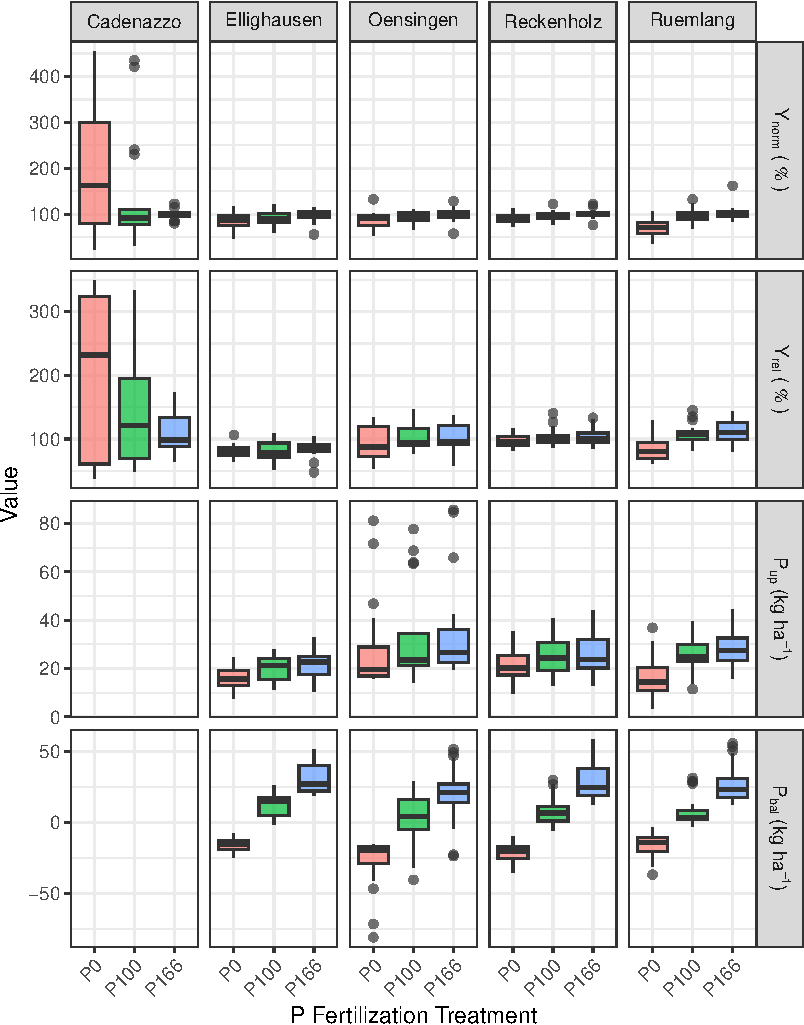
\includegraphics[keepaspectratio]{index_files/figure-pdf/fig-agronomic-responses-1.pdf}}

}

\caption{\label{fig-agronomic-responses}Agronomic response variables
across six P fertilization treatments and six experimental sites. Points
represent the median of replicates for each crop and year from
2017-2022.}

\end{figure}%

\textsubscript{Source:
\href{https://Andrapodon.github.io/Master-Thesis-P-kinetics/index.qmd.html}{Article
Notebook}}

\emph{(Placeholder for Figure X.1)}

\textbf{Yield Metrics (\(Y_{norm}\) and \(Y_{rel}\)):} Both yield
metrics, now displayed as percentages, showed a generally positive
response to P fertilization, especially at the lower treatment levels.
The site-normalized yield (\(Y_{norm}\)) clearly shows the response
relative to the site's potential for that year, with most yields
plateauing around the Norm (100\%) treatment. The national-normalized
yield (\(Y_{rel}\)) provides a broader context, showing how the yields
at each site compare to the national average. At some high-productivity
sites, even the zero-P treatment produced yields above the national
average (i.e., \textgreater{} 100\%), while at others, yields remained
below average even with high fertilization.

\textbf{P Uptake (\(P_{up}\)):} Phosphorus uptake by crops followed a
similar trend to yield, increasing with fertilization. However, unlike
yield, P uptake often continued to increase at the highest fertilization
levels. This suggests that at high P supply, plants engaged in ``luxury
consumption,'' taking up more P than was required for additional biomass
production.

\textbf{P Balance (\(P_{bal}\)):} The P balance showed a strong, linear
relationship with the fertilization treatment, which is expected by
definition. The Zero and Deficit treatments consistently resulted in a
negative P balance, indicating that crops were mining P from soil
reserves. The Norm treatment was generally close to a neutral balance,
while the Elevated and Surplus treatments led to a significant P
surplus, contributing to the accumulation of legacy P in the soil.

\subsubsection{Soil P Parameters as a Function of P
Fertilization}\label{soil-p-parameters-as-a-function-of-p-fertilization}

The different soil P test parameters, including the standard STP methods
and the newly derived kinetic parameters, all responded to the long-term
fertilization treatments (Figure X.2).

\phantomsection\label{cell-fig-soil-parameters}
\begin{figure}[H]

\centering{

\pandocbounded{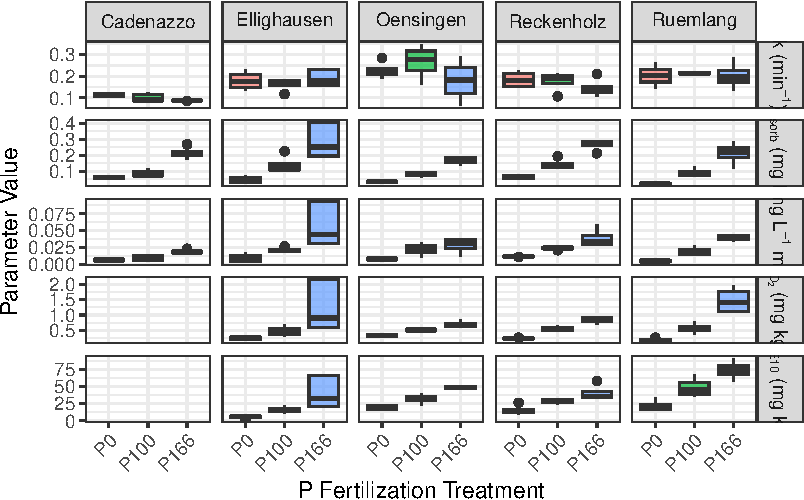
\includegraphics[keepaspectratio]{index_files/figure-pdf/fig-soil-parameters-1.pdf}}

}

\caption{\label{fig-soil-parameters}Soil P parameters across six P
fertilization treatments and six experimental sites. Points represent
the mean of replicates.}

\end{figure}%

\textsubscript{Source:
\href{https://Andrapodon.github.io/Master-Thesis-P-kinetics/index.qmd.html}{Article
Notebook}}

\emph{(Placeholder for Figure X.2)}

\textbf{Standard STPs (\(P_{CO_2}\) and \(P_{AAE10}\)):} Both standard
soil P tests showed a clear and consistent increase with rising P
fertilization levels across all sites. This confirms that both methods
are sensitive to changes in the soil P status resulting from long-term
management. The absolute values, however, differed significantly between
sites, reflecting the influence of soil properties like clay content and
pH on P retention.

\textbf{Kinetic Parameters (\(k\), \(P_{desorb}\), and \(J_0\)):} *
\textbf{Desorbable P (\(P_{desorb}\)):} This parameter, representing the
size of the readily desorbable P pool, behaved very similarly to the
standard STPs. It increased steadily with P fertilization, confirming
its role as a ``capacity'' indicator. * \textbf{Rate Constant (\(k\)):}
The rate constant, representing the speed of P release, showed a more
complex pattern. At most sites, \(k\) did not show a strong, consistent
trend with fertilization, or in some cases, it slightly decreased at
very high P levels. This suggests that while fertilization increases the
\emph{amount} of available P, it may not necessarily increase the
intrinsic \emph{release rate} from the soil matrix. * \textbf{Initial P
Flux (\(J_0\)):} As the product of \(P_{desorb}\) and \(k\), the initial
P flux integrates both the size of the pool and its release rate. It
showed a strong positive response to fertilization, driven primarily by
the increase in \(P_{desorb}\). This parameter effectively captures the
overall P-supplying power of the soil.

These initial observations suggest that while all P metrics are
sensitive to fertilization, the kinetic parameters, particularly the
rate constant \(k\), may provide unique information about the soil's P
dynamics that is not captured by static tests alone. The next section
will use formal statistical models to test these relationships.

\section{Discussion}\label{discussion}

\section{Conclusion}\label{conclusion}

\section{Acknowledgments}\label{acknowledgments}

\section{Legal Disclosure}\label{legal-disclosure}

\section*{References}\label{references}
\addcontentsline{toc}{section}{References}

\phantomsection\label{refs}
\begin{CSLReferences}{1}{0}
\bibitem[\citeproctext]{ref-knuth84}
Knuth, Donald E. 1984. {``Literate Programming.''} \emph{Comput. J.} 27
(2): 97--111. \url{https://doi.org/10.1093/comjnl/27.2.97}.

\end{CSLReferences}

\section{Appendix}\label{appendix}

\section{Supplements}\label{supplements}




\end{document}
